\documentclass{article}
\usepackage[table]{xcolor}
\usepackage{graphicx}
\begin{document}

Steven Avery
997694781
ECS 171 - Machine Learning
HW1
19 October 2014

\section*{Problem 1}
We want the size of the MPG bins to be the same, but with respect to the range of MPG, not with respect to the number of samples that fall into the bin. We avoid the latter situation because then we would have different models with the same MPG value in two different bins.

The thresholds for MPG:\\
$9 <= x <= 21.5$ : low\\
$21.5 < x < 34.1$ : medium\\
$34.1 <= x <= 46.6$ : high

\section*{Problem 2}
The best predictor of MPG is either horsepower, weight, or displacement. These all have a faily close relationship with MPG, but it's difficult to determine exactly which is the best from the graph.

\begin{center}
\includegraphics[scale=0.25]{problem2.png}
\end{center}

\section*{Problem 4}

The 22x7 matrix below is of RSS, which alternates between training and testing errors for the same order. The minimum RSS was training on order 1.
Using the testing error as the criteria for selecting the most informative feature, the minimum RSS generated at the 1st order was on weight.

\begin{center}
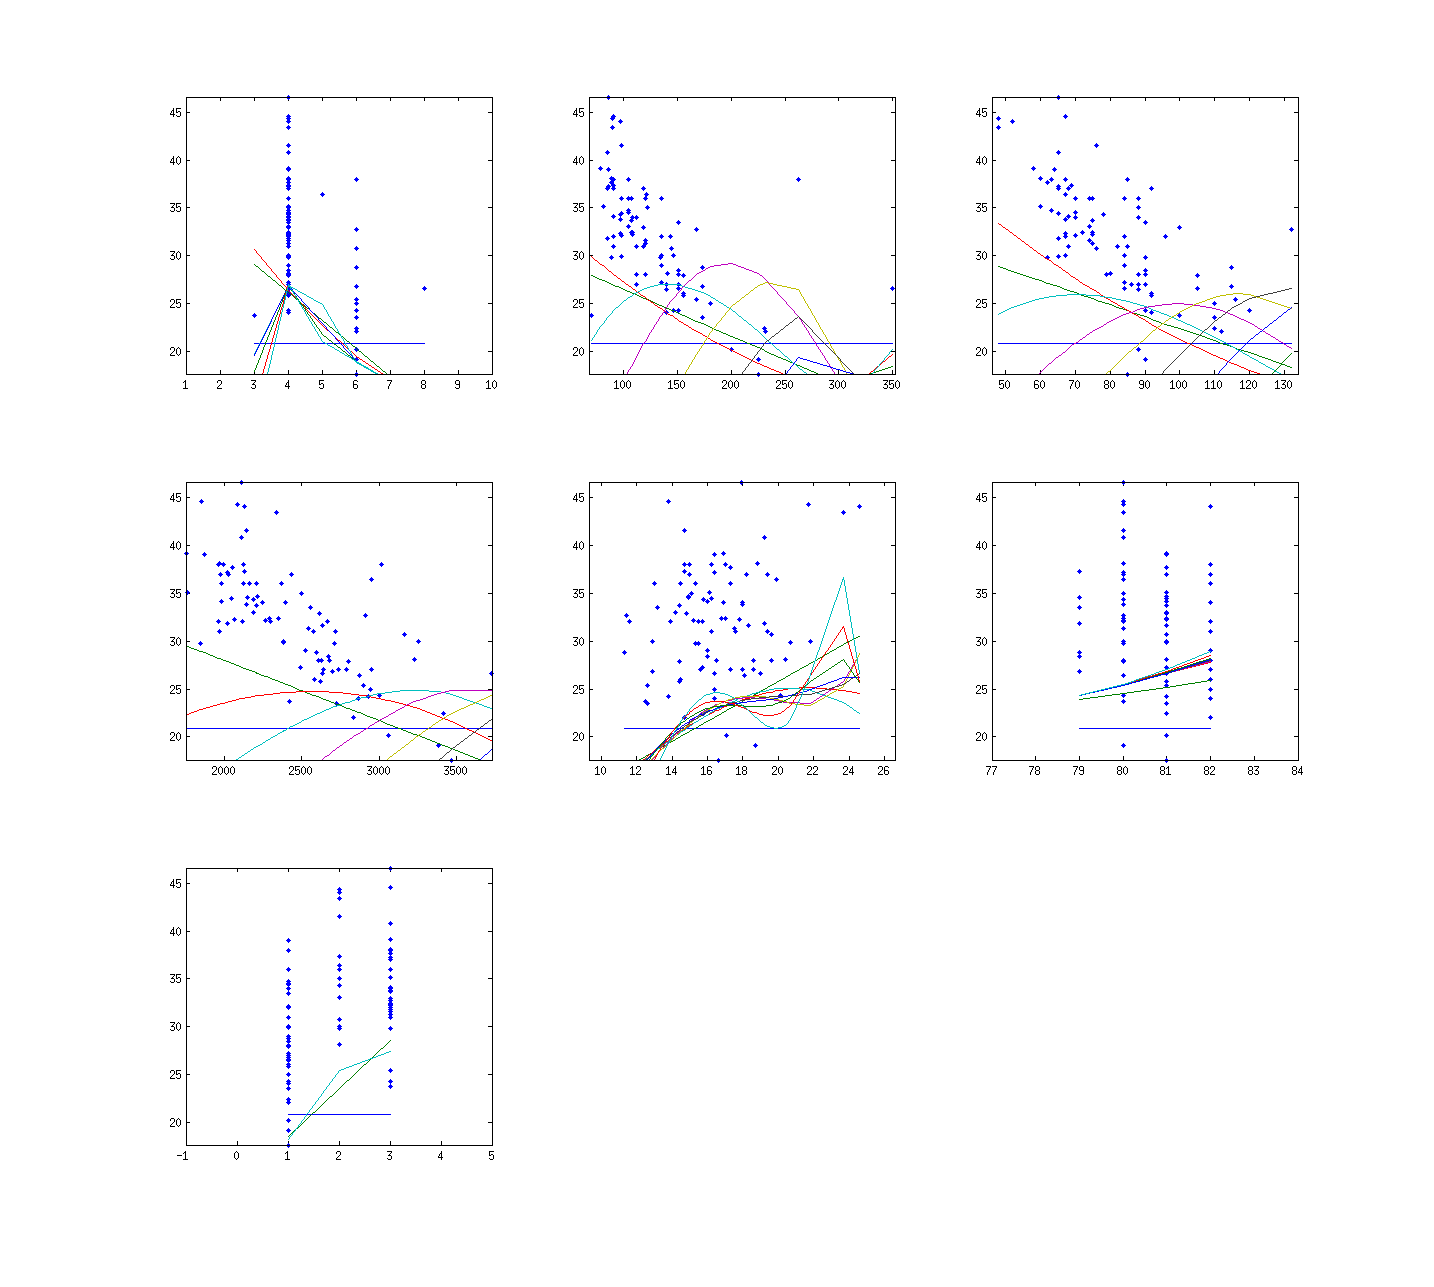
\includegraphics[scale=0.25]{problem4.png}
\end{center}

\begin{center}
\rowcolors{1}{white}{gray}
\begin{tabular}{rlllllll}
 & cylinders & displacement & horsepower & weight & acceleration & model year & origin \\ 
training - 0 & 11983.29 & 11983.29 & 11983.29 & 11983.29 & 11983.29 & 11983.29 & 11983.29 \\
testing & 14499.05 & 14499.05 & 14499.05 & 14499.05 & 14499.05 & 14499.05 & 14499.05 \\
training - 1 & 4031.46 & 3470.14 & 4302.56 & 2739.64 & 9524.88 & 10937.95 & 7830.39 \\
testing & 6822.59 & 6447.29 & 6793.14 & 6122.51 & 12202.26 & 7527.47 & 10130.01 \\
training - 2 & 3962.68 & 2923.52 & 3251.82 & 7327.67 & 9248.21 & 10915.05 & 7554.04 \\
testing & 6776.98 & 5930.25 & 5568.98 & 8995.89 & 12155.59 & 6111.40 & 10265.63 \\
training - 3 & 3541.58 & 6530.20 & 5133.35 & 20011.94 & 9228.49 & 10916.79 & 7554.04 \\
testing & 6318.95 & 7991.67 & 7453.67 & 18194.52 & 12264.67 & 6093.87 & 10265.63 \\
training - 4 & 3533.21 & 25741.30 & 12948.62 & 39636.51 & 9019.55 & 10918.46 & 7554.04 \\
testing & 6342.71 & 21958.28 & 14902.22 & 34039.55 & 11957.19 & 6086.83 & 10265.63 \\
training - 5 & 3533.21 & 58497.95 & 27839.59 & 60314.42 & 9074.87 & 10920.24 & 7554.04 \\
testing & 6342.71 & 50283.24 & 28586.61 & 52091.89 & 11972.77 & 6082.49 & 10265.63 \\
training - 6 & 3533.21 & 82306.81 & 49060.99 & 77642.69 & 9206.53 & 10922.35 & 7554.04 \\
testing & 6342.71 & 73535.92 & 46747.54 & 67388.91 & 11989.89 & 6071.92 & 10265.63 \\
training - 7 & 3533.21 & 95354.36 & 72263.96 & 90698.83 & 9270.51 & 10925.04 & 7554.04 \\
testing & 6342.71 & 85217.65 & 65149.35 & 78230.64 & 11956.00 & 6045.16 & 10265.63 \\
training - 8 & 3543.81 & 103175.83 & 91379.90 & 100241.52 & 9454.25 & 10928.62 & 7554.04 \\
testing & 6351.84 & 90596.75 & 79018.90 & 85250.91 & 11908.95 & 5991.73 & 10265.63 \\
training - 9 & 3612.60 & 108580.21 & 104389.86 & 107266.27 & 9946.51 & 10933.40 & 7554.04 \\
testing & 6380.30 & 93183.75 & 87300.85 & 89628.07 & 11917.88 & 5901.70 & 10265.63 \\
training - 10 & 3729.88 & 112642.75 & 112753.45 & 112552.83 & 11006.78 & 10939.79 & 7554.04 \\
testing & 6426.41 & 94510.53 & 91741.02 & 92330.37 & 12129.28 & 5767.93 & 10265.63 \\
\end{tabular}
\end{center}


\section*{Problem 5}

\begin{center}
\begin{tabular}{rll}
order & training & test \\
\\
0 &	11983.2958666667 & 14499.0575342222 \\
1 & 2138.01747578572 & 3069.02396910692 \\
2 & 2662.77880441783 & 2596357829.01521 \\
\end{tabular}
\end{center}

\section*{Problem 6}
I couldn't get my cost function to converge. It would seem like it was converging up to a certain point, and then continue in a linear fashion.
My code working on this is in GetCost, GradientDescent, and problem6.

\section*{Problem 7}
Using only the OLS approach:
Our expected value is generated from the problem's proposed vehicle and the weights generated from problem 5.
Somehow, I generated 9945 MPG, which would definitely qualify this vehicle in the high MPG category.

\end{document}
